\documentclass{beamer}

\title{Analyse des enlèvements}
\author{Fournisseur: \textbf{<< provider >>}}
\titlegraphic{\vspace*{0.5cm} 
\includegraphics[width=5cm]{images/leclerc}}
\date{<< periode >> << annee >>}

\setlength{\parskip}{0.2cm}
\usepackage[font=tiny]{caption}

\begin{document}
    \begin{frame}
        \titlepage
    \end{frame}

    \begin{frame}
        \frametitle{Table des matières}
        \tableofcontents
    \end{frame}

    \section{Introduction}

    \begin{frame}
        \tiny
        \frametitle{Introduction}
        Ce rapport traite les données du mois de << periode >> << annee >>. Il analyse en détail les achats de nos points de vente.\par

        Quelques informations clefs :

        \begin{itemize}
            \item{Le \textbf{CA} total du mois dernier s’élève à \textbf{<< ca_total_mois|number(2) >>€}.}
            \item{\textbf{<< nb_uvc_mois|number >> UVC} ont été commandés le mois dernier par nos points de vente}
            \item{\textbf{<< nb_ref_mois|number >> références} articles ont été commandées}
            \item{\textbf{<< nb_magasins|number >> points de vente} ont commandé vos articles}
            \item{Voici la liste des points de vente qui n’ont pas réalisé de commande sur vos références le mois dernier : << ', '.join(list_mag_nop) >>.}
        \end{itemize}

        Dans la première partie, l’analyse est détaillée par point de vente.\par
        Dans la deuxième partie, l’analyse est détaillée par mode de gestion.\par
        Dans la troisième partie, l’analyse est détaillée par article.\par
        Pour rappel, vous avez souscrit au contrat << nom_contrat >> le << date_contrat >> pour une mise à disposition des données mensuelles détaillées à l’article et par point de vente.\par
    \end{frame}

    \section{Analyse des points de vente}

    \begin{frame}
        \tiny
        \frametitle{Analyse des points de vente}

        Les visualisations ci-dessous représente le CA (PERMANENT + NON PERMANENT) par points de vente.\par

        <@ set column_count = 3  @>

        <@ for row in assets.ca|batch(column_count) @>
            \begin{columns}
                <@ for img in row @>
                    \column{<< 1 / column_count >>\textwidth}
                        \centering
                        \begin{figure}[h]
                            \centering
                            \includegraphics[width=1\textwidth]{<< img >>}
                        \end{figure}
                <@ endfor @>
            \end{columns}
        <@ endfor @>

        Le point de vente avec le CA le plus élevé à \textbf{<< magasin_ca_plus_eleve.ca|number >>€}, est \textbf{<< magasin_ca_plus_eleve.nom_magasin >>}.\par
        Le point de vente \textbf{<< magasin_ca_moins_eleve.nom_magasin >>} avec \textbf{<< magasin_ca_moins_eleve.ca|number >>€} représente le plus petit CA du mois.\par
        La visualisation ci-dessus présente la somme des quantités commandées (PERMANENT + NON PERMANENT) par point de vente.\par
        \textbf{<< magasin_uvc_plus_eleve.nom_magasin >>} est le point de vente ayant commandé le plus d’UVC : \textbf{<< magasin_uvc_plus_eleve.quantite|number >> UVC au mois de ???}.\par
        Le point de vente \textbf{<< magasin_uvc_moins_eleve.nom_magasin >>} avec : \textbf{<< magasin_uvc_moins_eleve.quantite|number >> UVC} représente la plus faible quantité du mois.\par
    \end{frame}

    \subsection{Localisation}
    \subsection{Activité}

    \begin{frame}
        \tiny
        \frametitle{Localisation}

        \begin{columns}
            \column{0.66\textwidth}
                La visualisation ci-contre présente la répartition du CA du mois dernier par localisation :

                \begin{itemize}
                    <@ for localisation, part_ca in ca_par_localisation.items() @>
                        \item{Les points de vente \textbf{<< localisation >>} représentent \textbf{<< part_ca|number(1) >>\%} du CA}
                    <@ endfor @>
                \end{itemize}

            \column{0.33\textwidth}
                \centering

                \begin{figure}[h]
                    \centering
                    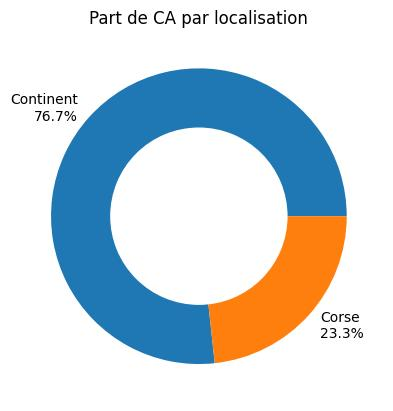
\includegraphics[width=1\textwidth]{assets/ca_par_localisation}
                \end{figure}
        \end{columns}

        {\hskip-3em\usebeamerfont{frametitle}\usebeamercolor[fg]{frametitle} Activité}

        \begin{columns}
            \column{0.33\textwidth}
                \centering

                \begin{figure}[h]
                    \centering
                    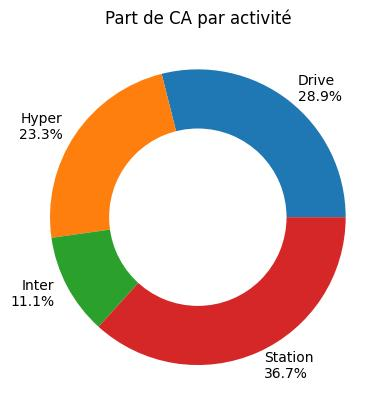
\includegraphics[width=1\textwidth]{assets/ca_par_activite}
                \end{figure}

            \column{0.66\textwidth}
                La visualisation ci-contre présente la répartition du CA par activité :

                \begin{itemize}
                    <@ for activite, part_ca in ca_par_activite.items() @>
                        \item{Les points de vente \textbf{<< activite >>} représentent \textbf{<< part_ca|number(1) >>\%} du CA}
                    <@ endfor @>
                \end{itemize}
        \end{columns}
    \end{frame}

    \section{Analyse du mode de gestion}

    \begin{frame}
        \tiny
        \frametitle{Analyse du mode de gestion}

        \begin{columns}
            \column{0.66\textwidth}
            La visualisation ci-contre présente la répartition des modes de gestion pour les CA du mois :

            \begin{itemize}
                \item{Les points de vente \textbf{<< localisation >>} représentent \textbf{<< part_ca|number(1) >>\%} du CA}
            \end{itemize}

            \column{0.33\textwidth}
            \centering

            \begin{figure}[h]
                \centering
                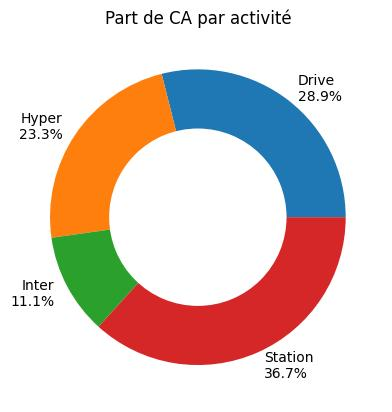
\includegraphics[width=1\textwidth]{assets/ca_par_mode_de_gestion}
            \end{figure}
        \end{columns}

        D’après ces visualisations {4} points de vente ont commandé uniquement en PERMANENT.
    \end{frame}

    \subsection{Non permanent}

    \begin{frame}
    \end{frame}

    \subsection{Permanent}

    \begin{frame}
    \end{frame}

    \section{Analyse par article}
    \subsection{Articles les plus commandés}

    \begin{frame}
    \end{frame}

    \subsection{Articles les moins commandés}

    \begin{frame}
    \end{frame}

\end{document}
